\documentclass[hidelinks,12pt,a4paper,openright,twoside]{book}
\usepackage[italian]{babel}
\usepackage[utf8]{inputenc}
\usepackage{fourier}

% Images
\usepackage{graphicx}
\usepackage{caption}
\usepackage{subcaption}
\usepackage{float}
\graphicspath{ {../Images} }

% Stop hyphenation
\usepackage[none]{hyphenat}

% Background page image.
\usepackage{eso-pic}
\usepackage[top=2cm, bottom=2cm, outer=0cm, inner=0cm]{geometry}

% To hide images
\usepackage[allfiguresdraft]{draftfigure}

% To color text parts
\usepackage{xcolor}

% Adjust margins
\usepackage{changepage}

% License
\usepackage[
type={CC},
modifier={by-nc-sa},
version={4.0},
]{doclicense}

\begin{document}
	
	% Remove page number
	\pagestyle{empty}
	
	% Album Cover
	\begin{center}
		\vspace*{15mm}
		\fboxrule=4pt{
		\fbox{ %                  height                                width
			\begin{minipage}[l] [\dimexpr 0.150\textwidth \relax] [t] {\dimexpr .460\textwidth \relax}
				\vspace{5mm}
				\centering{\large \textbf{Album sulle opere del Museo Civico\\}}
				\bigskip
				Alice Balestieri \\
				Francesco Rombaldoni
			\end{minipage}
			}
		}
	\end{center}
	
	% Background image
	\AddToShipoutPictureBG*{\includegraphics[draft=false, width=\paperwidth,height=\paperheight]{example-image}}
	%\clearpage
	
	\newpage
	
	%--------- Page 1 ----------
		
			%  Mengaroni_Ferruccio-Medusa
			\begin{minipage}{0.5\linewidth}
				\begin{center}
					\setdf{content={\textcolor{white}{\hspace{25mm} \Large \#1}}}
					\colorbox{black}{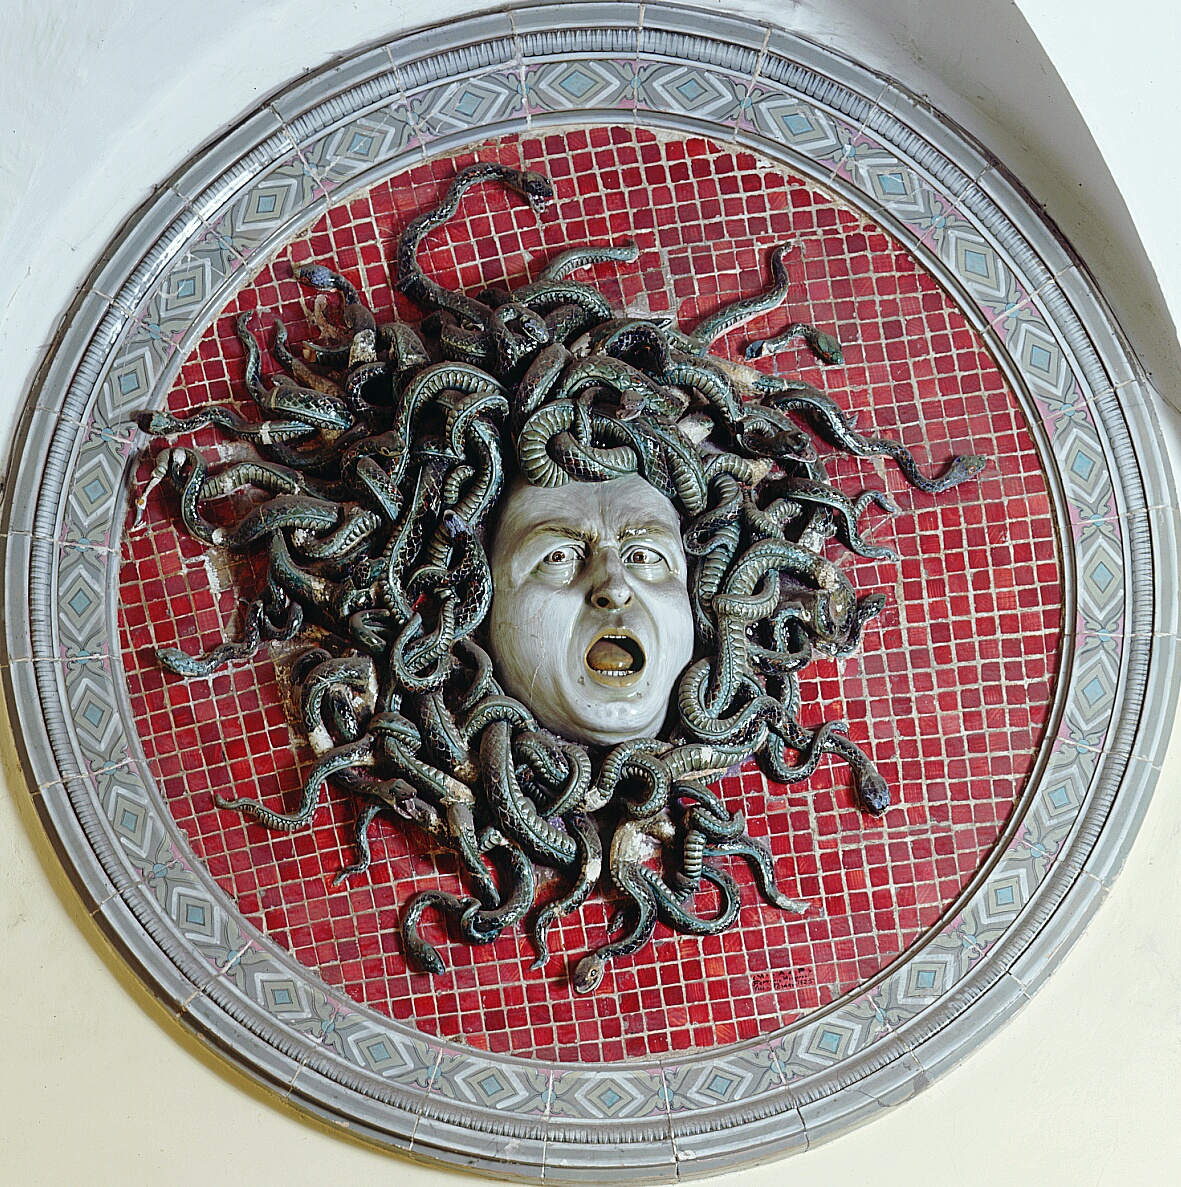
\includegraphics[scale = 1.2]{Mengaroni_Ferruccio-Medusa.jpg}}
				\end{center}
				\begin{center}
					\begin{minipage}{\linewidth}
						\raggedright
						"La Medusa" accoglie i visitatori introducendoli alle sale espositive; si tratta dell'ultima opera di Ferruccio Mengaroni.\\
						L'imponente Medusa ritrae i lineamenti dell'artista pesarese: la leggenda narra che, per riprodurre il proprio volto, egli si fosse servito di uno specchio che poi si ruppe.
					\end{minipage}
			\end{center}
			\end{minipage}
		
		\vspace{10mm}
		
			\begin{adjustwidth}{0mm}{5mm}
				\raggedleft{
				% Bellini_Giovanni-Incoronazione_della_Vergine
				\begin{minipage}{0.5\linewidth}
					\begin{center}
						\setdf{content={\textcolor{white}{\hspace{25mm} \Large \#2}}}
						\colorbox{black}{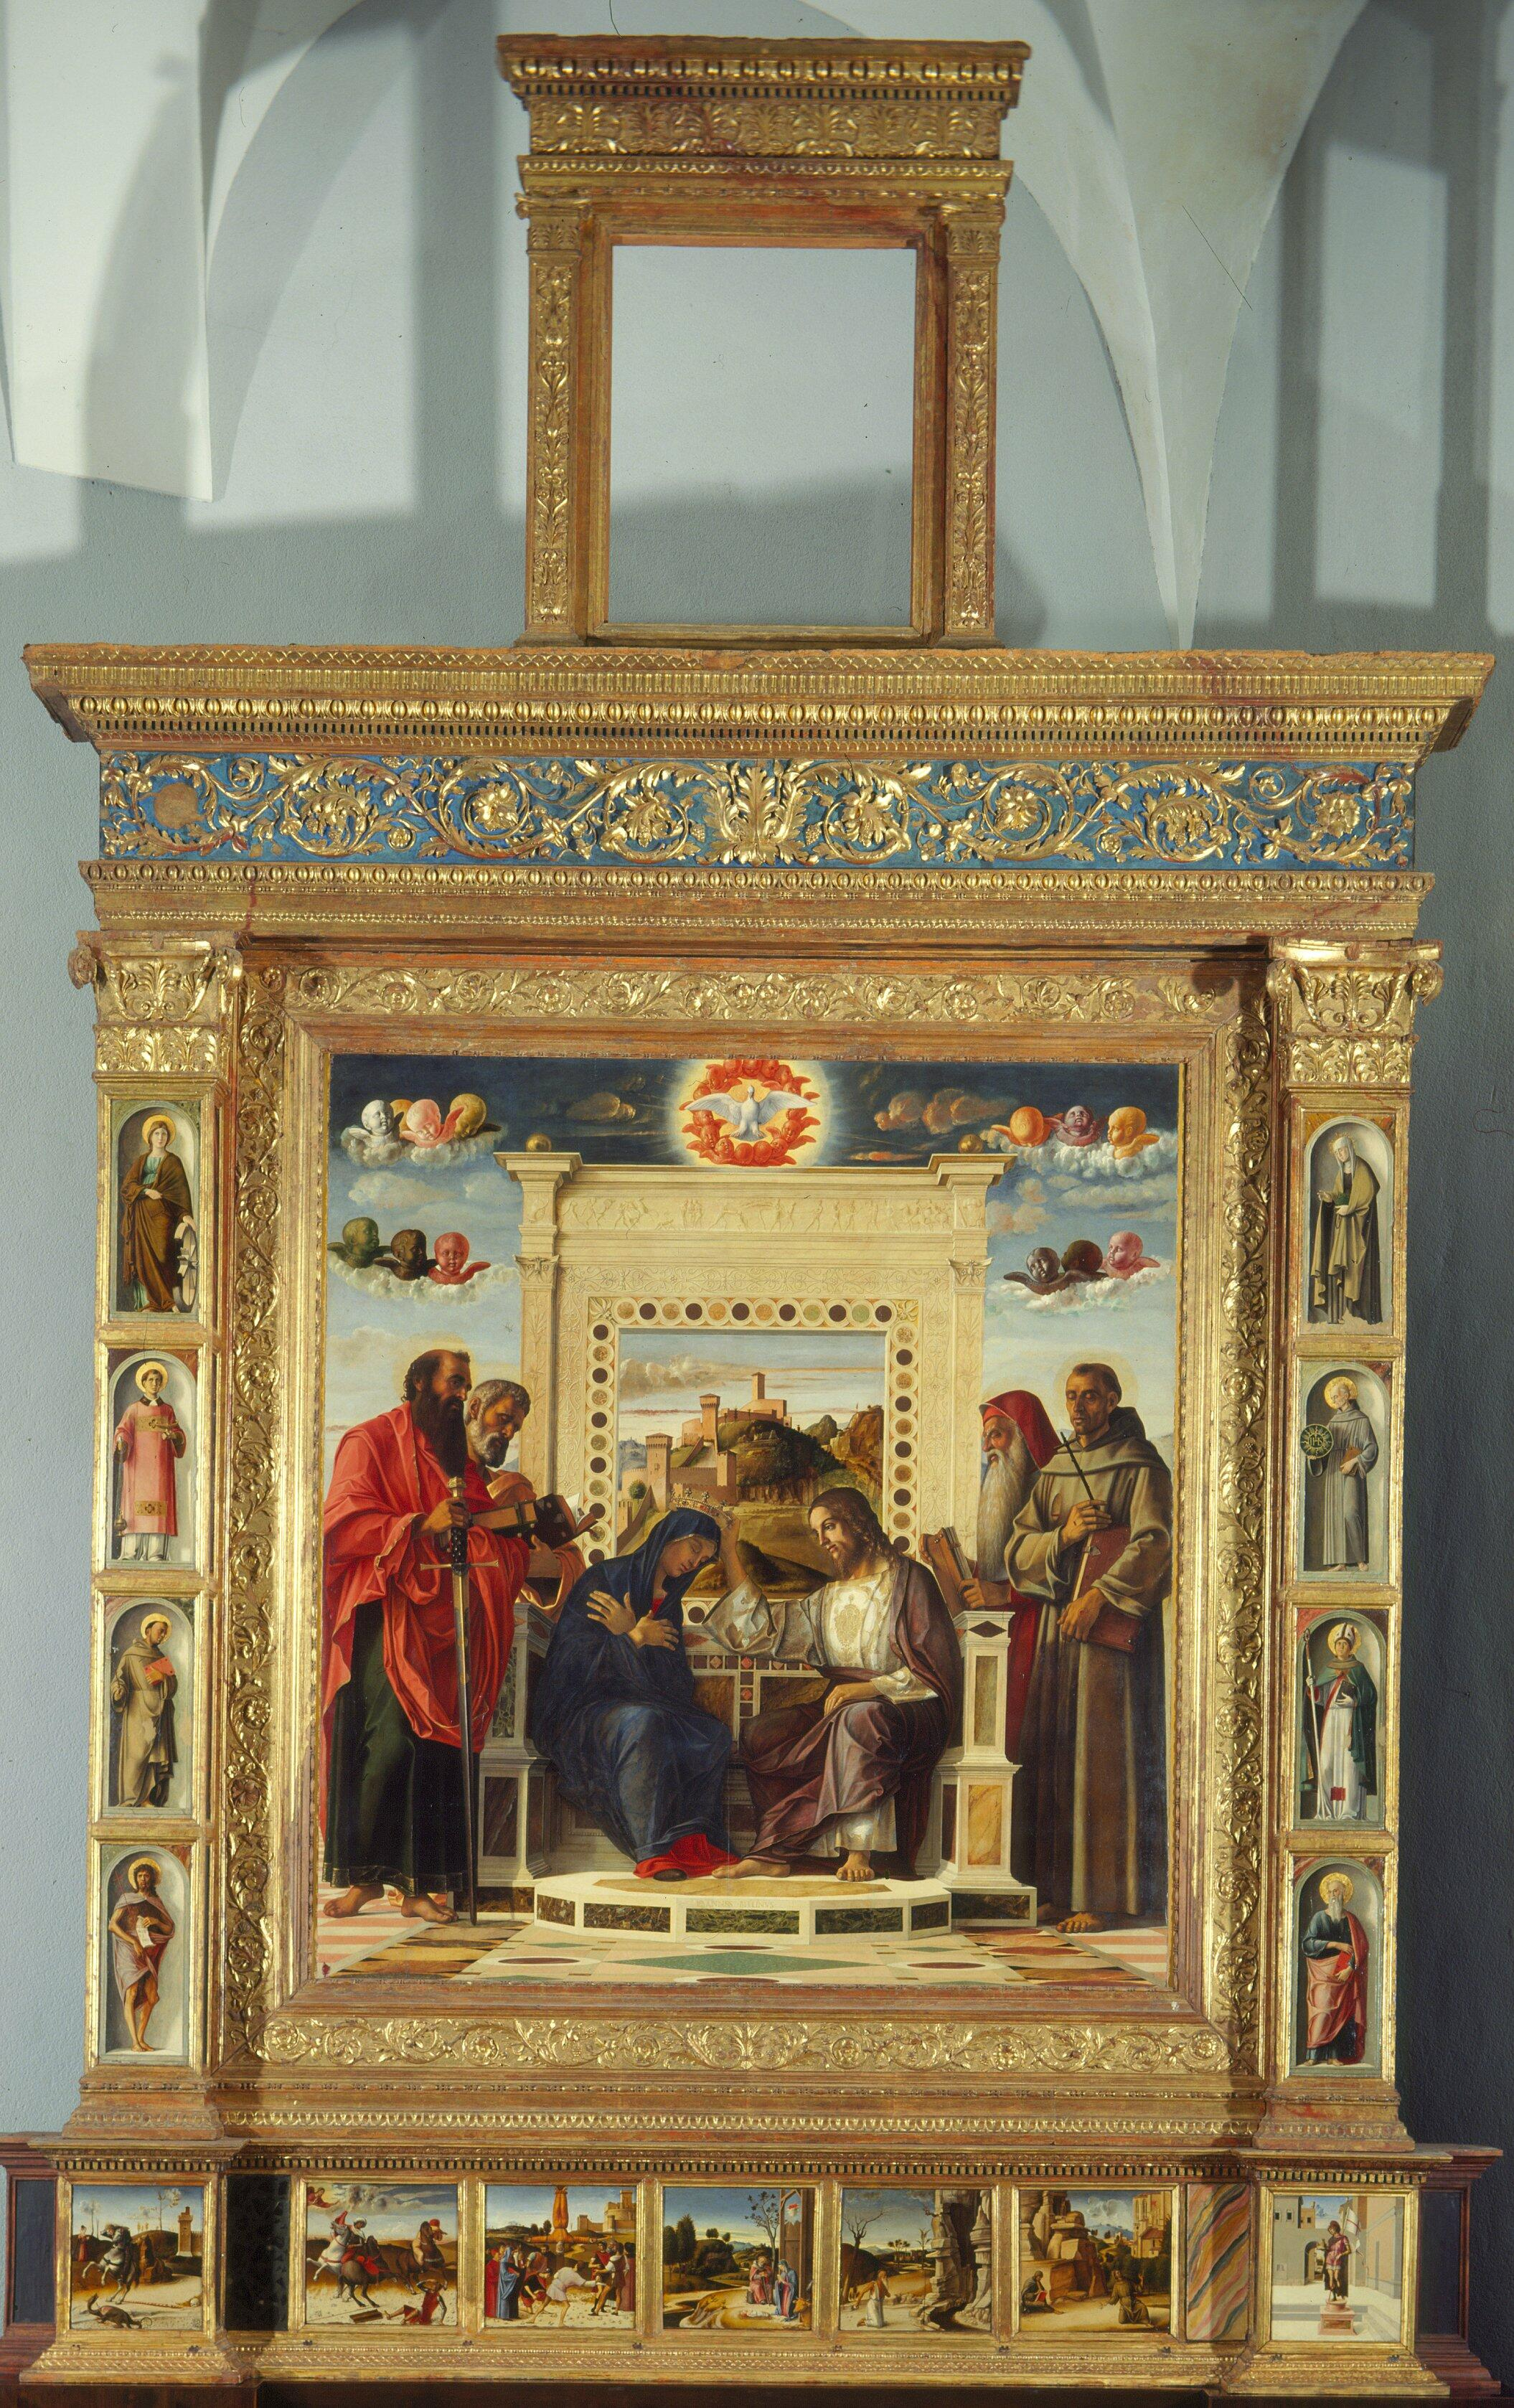
\includegraphics[scale=0.085]{Bellini_Giovanni-Incoronazione_della_Vergine.jpg}}
					\end{center}
			
					\begin{center}
					\begin{minipage}{\linewidth}
						\raggedright
						La pala, uno straordinario lavoro di carpenteria, costruito in vista, di un estrema semplicità di montaggio e tenuto insieme mirabilmente da pochi cavicchi di legno, fu dipinta per l'altare maggiore della chiesa di San Francesco a Pesaro.
					\end{minipage}
				\end{center}
			\end{minipage}
		}
	\end{adjustwidth}

	% Background image
	\AddToShipoutPictureBG*{\includegraphics[draft=false, width=\paperwidth,height=\paperheight]{example-image-plain}}
	
	\newpage
		
	%--------- Page 2 ----------
	
	% First Line
	\begin{minipage}{\linewidth}
		
		%Vitale da Bologna - Sant'Ambrogio in trono
		\begin{minipage}{0.4\linewidth}
			\begin{center}
				\setdf{content={\textcolor{white}{\hspace{18mm} \Large \#3}}}
				\colorbox{black}{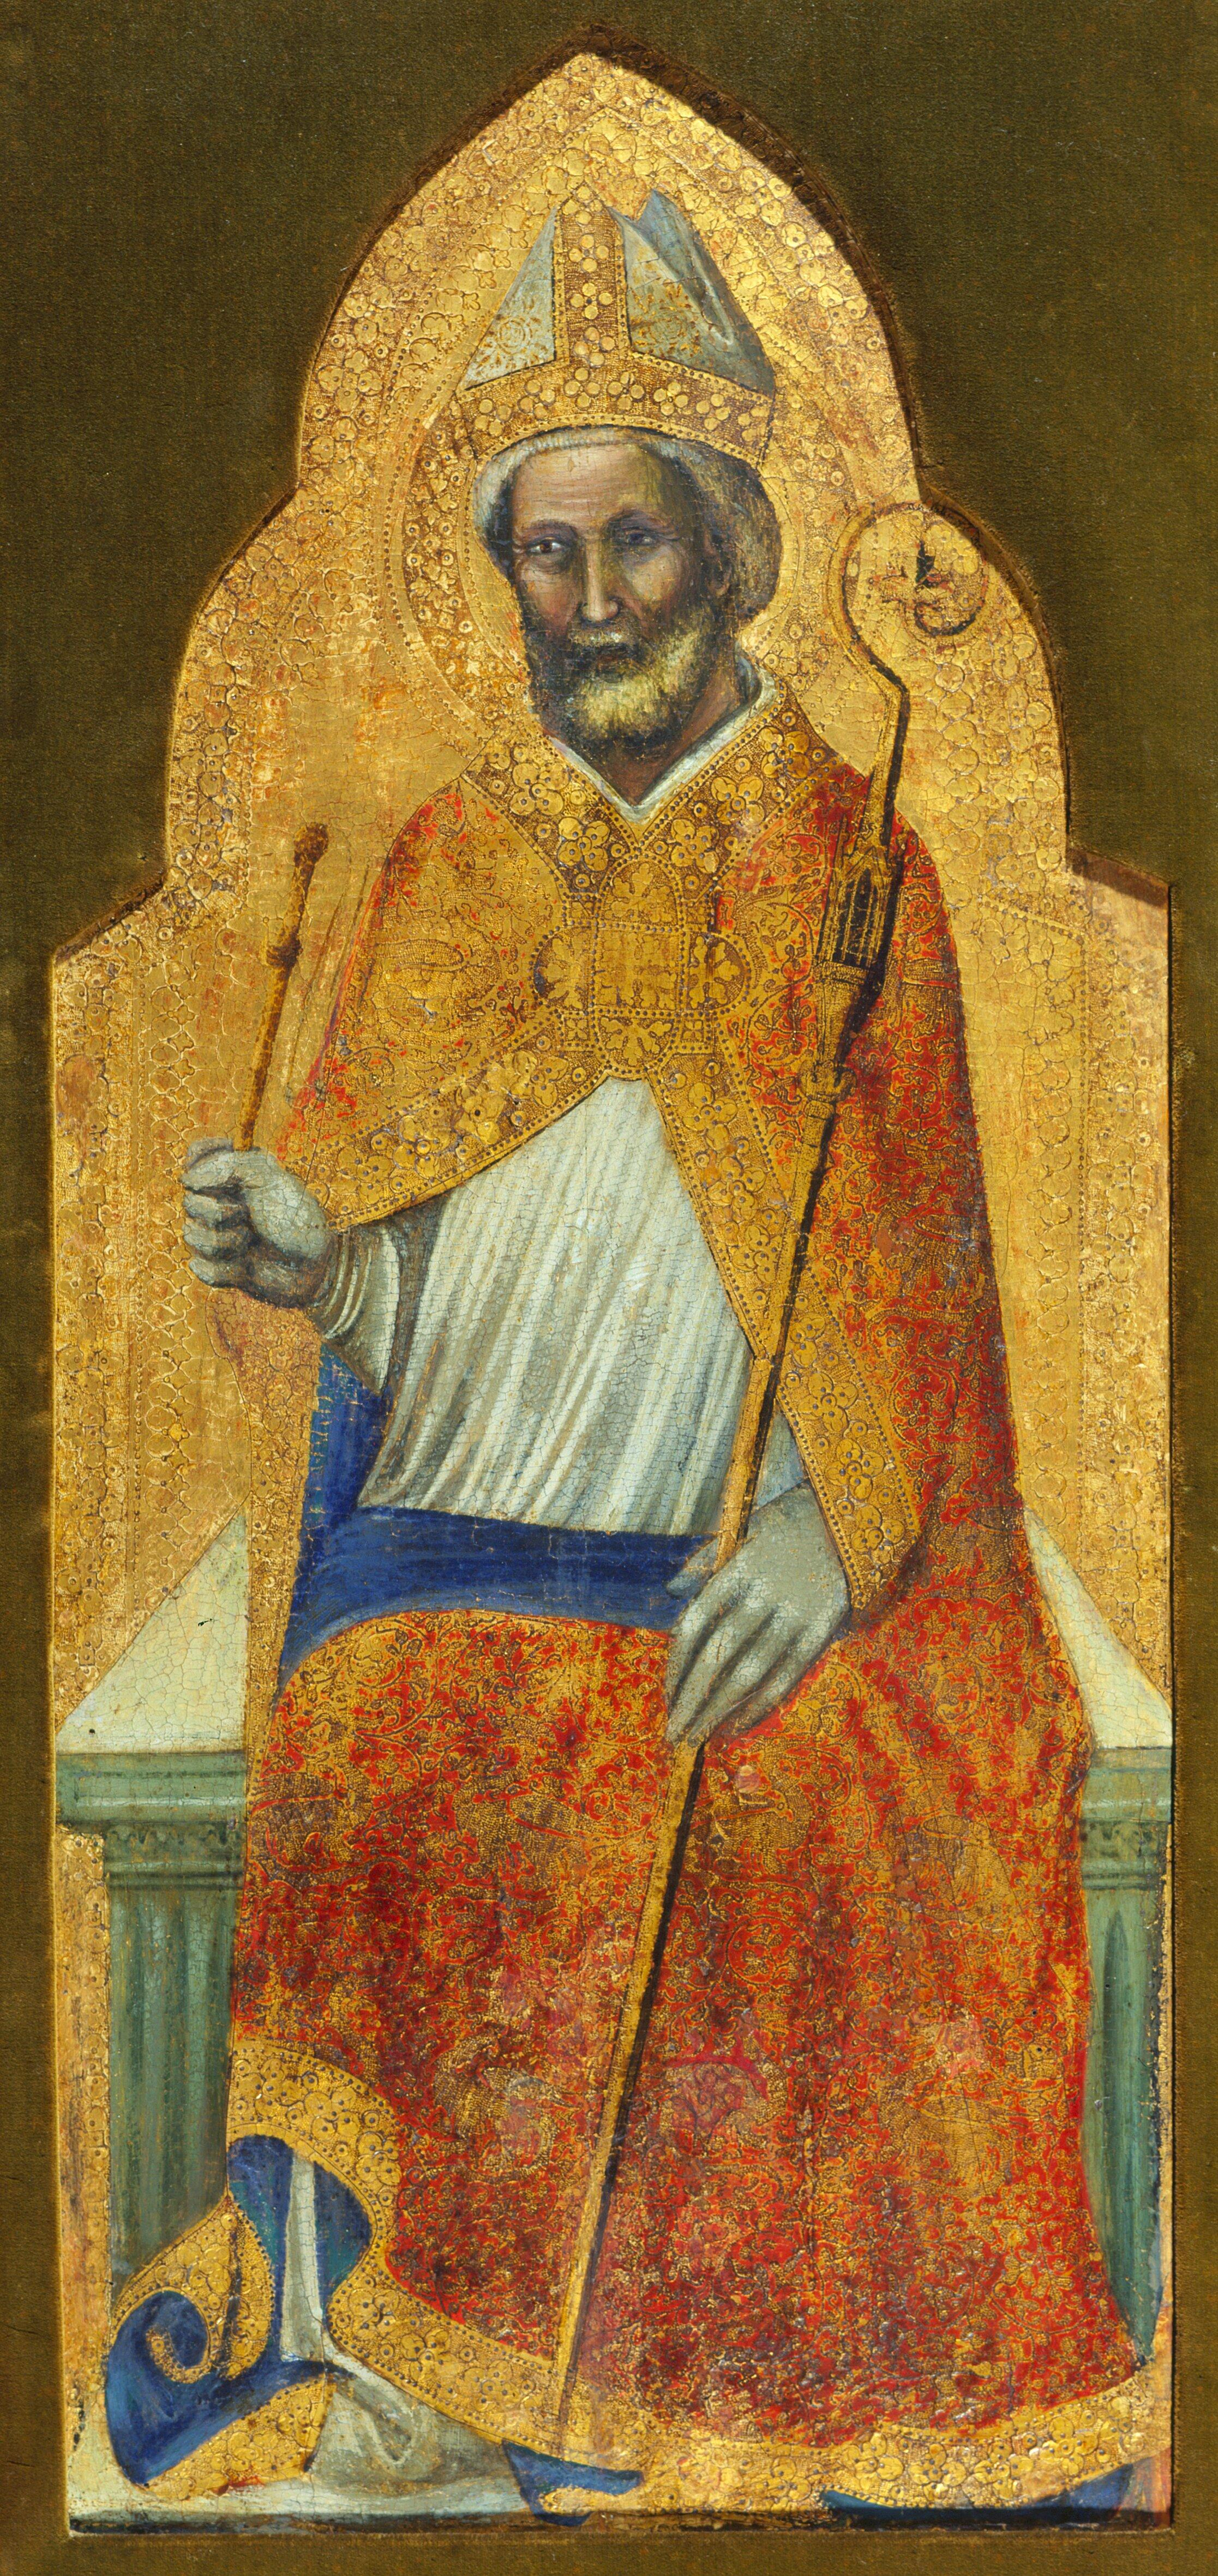
\includegraphics[scale=0.06]{Vitale_da_Bologna-Santo_Ambrogio_in_trono.jpg}}
			\end{center}
		
			\begin{center}
				\begin{minipage}{\linewidth}
					\raggedright
					Nonostante sia stata sottoposta in tempi recenti a restauro, la tavola presenta ancora nella superficie pittorica varie abrasioni, dovute forse ad antichi restauri, che ne compromettono in parte la leggibilità. Ciò è evidente soprattutto nella zona del viso del santo, fortemente consunta e priva ormai, nella resa dell'incarnato, di quelle connotazioni più morbidamente sfumate che sono tipiche dell'arte vitalesca.
				\end{minipage}
			\end{center}
		\end{minipage}
		
		\begin{adjustwidth}{0mm}{20mm}
		\raggedleft{
		% Desani Pietro - Rebecca ed Eleazar
		\begin{minipage}{0.4\linewidth}
			\begin{center}
				\setdf{content={\textcolor{white}{\hspace{15mm} \Large \#4}}}
				\colorbox{black}{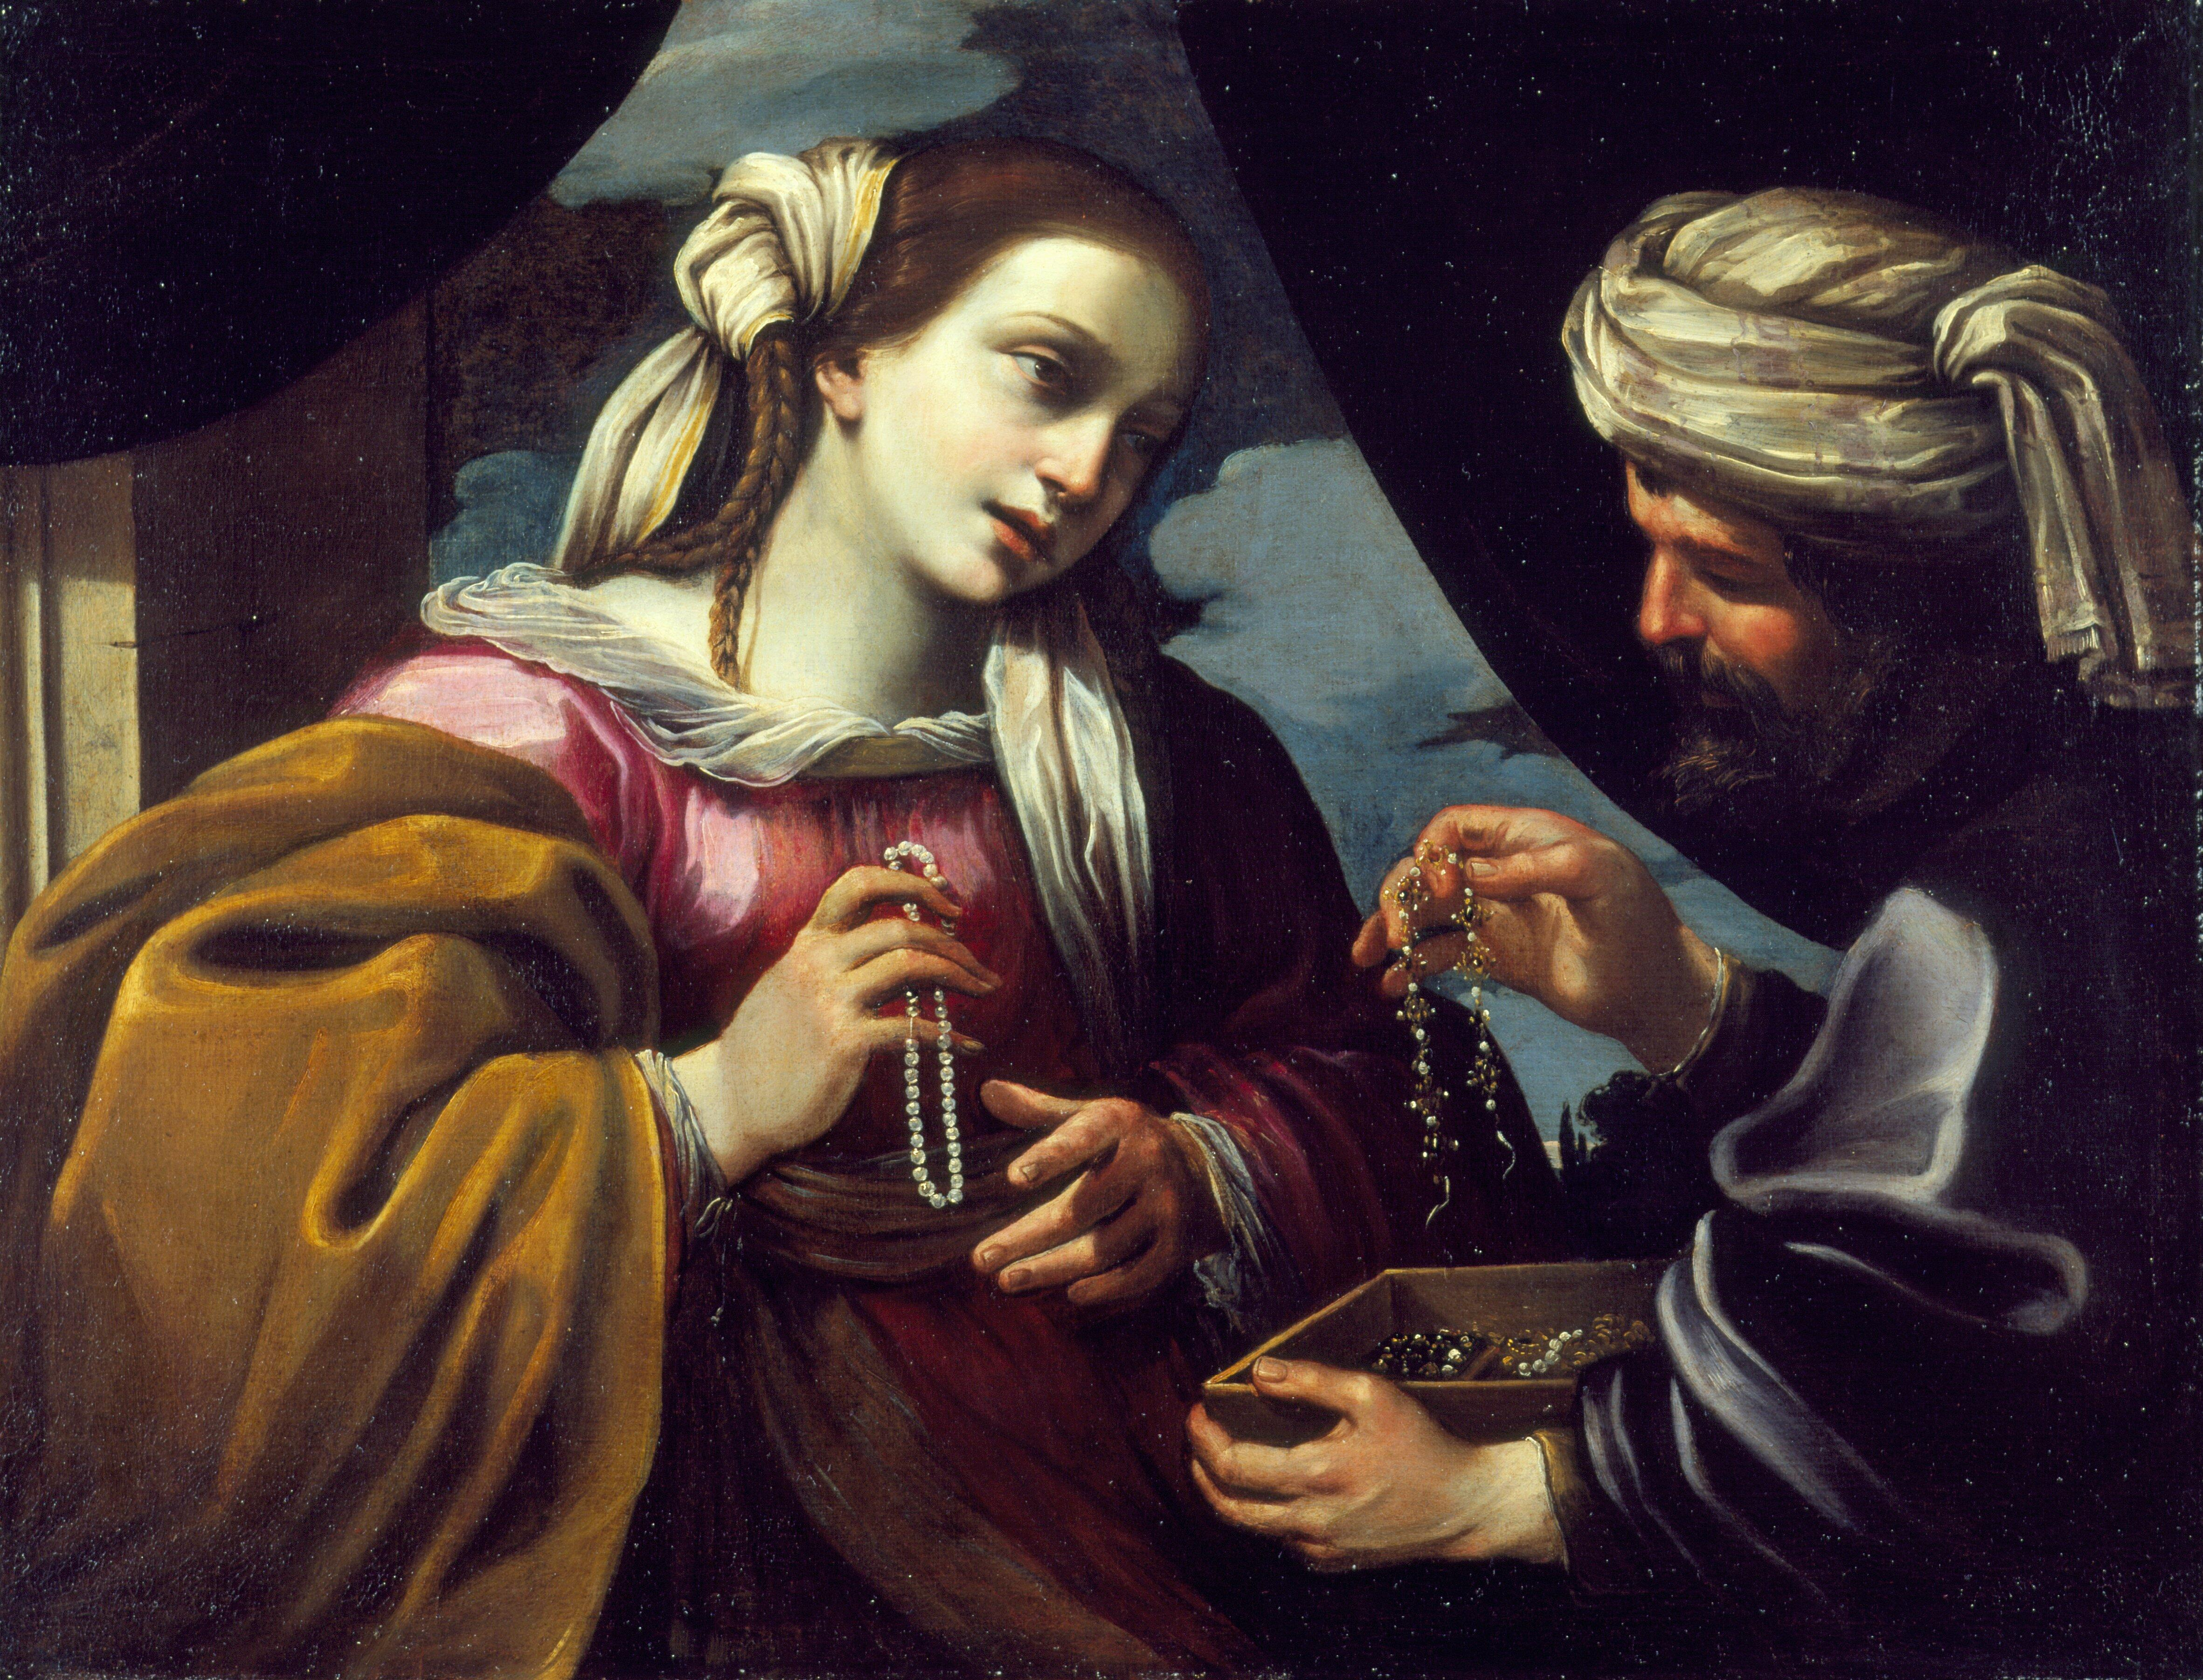
\includegraphics[scale = 0.05]{Desani_Pietro-Rebecca_ed_Eleazar.jpg}}
			\end{center}
		
			\begin{minipage}{\linewidth}
				\begin{center}
					\raggedright
					Il fido Eleazar, mandato in Mesopotamia da Abramo per cercare una sposa per suo figlio Isacco incontra a un pozzo una fanciulla che lo disseta e alla quale consegna i gioielli che gli sono stati dati per l'eletta.\\
					Secondo quanto si apprende dalle ricerche condotte in questa occasione da Barbara Ghelfi, il dipinto venne ereditato nel 1806 da Maria Malvezzi: nell'occasione veniva detto "Due mezze figure che contrattano delle gioie, d´uno stile che somiglia il Tiarini".
				\end{center}
			\end{minipage}
			
		\end{minipage}
	}
\end{adjustwidth}
	\end{minipage}

	
\end{document}